%%%%%%%%%%%%%%%%%%%%%%%%%%%%%%%%%%%%%%%%%%%%%%%%%%%%%%%%%%%%%%%%%%%%%%%%
\chapter{Methods for Fetal Brain Segmentation} \label{chap:MethodsForFetalBrainSegmentation}
%%%%%%%%%%%%%%%%%%%%%%%%%%%%%%%%%%%%%%%%%%%%%%%%%%%%%%%%%%%%%%%%%%%%%%%%
\vspace{1cm}

The Fetal Tissue Annotation Challenge (FeTA) \cite{FeTA2024} was born in 2020, and joined the International Conference on Medical Image Computing and Computer-Assisted Intervention (\textsc{miccai}) \cite{MICCAI} in 2021. Up to now, four editions have been organized (in 2020, 2021, 2022, and 2023), with increasing participation and interest from the medical imaging community. The main contributions of the FeTA challenge are the creation of a benchmark dataset for fetal brain MRI segmentation and biometry, and the promotion of the development of algorithms for the automatic segmentation of fetal brain tissues.

The main task in FeTA is the segmentation of brain tissues in fetal MRI, which is a challenging problem due to the low contrast between tissues, the presence of noise, and the variability in the shape and size of the fetal brain. The dataset used in the challenge is composed of 3D super-resolution (SR) reconstructions of 2D fetal brain MRI images. Participants are asked to segment the fetal brain into seven tissues. The performance is evaluated using different metrics, such as the Dice similarity coefficient between the predicted and ground truth segmentations. \cite{FeTA2024_paper}

\section{Domain Generalization}

\section{Atlas-based Methods}

\section{The FeTA Challenge}

The first edition of the FeTA challenge was organized in 2020, by Payette et al.\ \cite{FeTA2020_review}. The challenge consisted in segmenting fetal brain MRI T2w images. The initial FeTA dataset comprised 40 super-resolution (SR) reconstructions with manual segmentations for training and 10 SR reconstructions without manual segmentation for validation, encompassing both pathological and non-pathological cases. The gestational age (GA) range spanned from 20 to 33 weeks. The scans were acquired in This dataset established a standard in fetal brain tissue parcellation---according to a seven-tissues protocol previously introduced in \cite{Payette2020}---that would be used in all the following FeTA editions. The seven tissue types are: external cerebrospinal fluid (CSF), cortical gray matter (GM), white matter (WM), ventricles, cerebellum, deep gray matter, and brainstem.

Four research groups participated, submitting a total of ten algorithms. Nine out of ten used deep learning methods (eight of which were based on 2D and 3D U-Nets), and one used a multi-atlas segmentation method. The assessment of the results was carried out using the Dice similarity coefficient (DSC), the volume similarity (VS), and the Hausdorff 95 distance (HD95). The use of three metrics helps to reduce the reliance on any one metric, which may be misleading in the evaluation of the algorithms. In fact, the authors admit that manual segmentations included in both the training and testing dataset were not perfect, and therefore there are mislabeled voxels, especially in low-resolution scans \cite{FeTA2021_review}. All the algortihms had more or less the same issues in segmenting the CSF---especially for the pathological cases, because of not clear tissue boundaries---and the GM, because of its rapidly changing structure. The best performing method was a 3D U-Net made up by the combination of three 2D U-Nets, one per direction (sagittal, coronal, and axial). It is worth noting that the multi-atlas segmentation method performed better than the deep learning methods when the quality of the SR was poor. This is because such method can leverage its prior knowledge even if the structure is not clear in the image.

The dataset used in the first FeTA edition had important limitations:
\begin{itemize}
    \item Manual segmentations were based on a single segmentation due to time and resource limitations, without consensus delineation.
    \item The data were from one single center, the University Children's Hospital Zurich (Kispi), thus limiting the generalizability of the results.
    \item The images had varying quality grades, with younger GAs and pathological cases often having lower quality.
\end{itemize}

\subsection{FeTA 2021}

The 2021 edition of the FeTA challenge \cite{FeTA2021_review, FeTA2021} was the first to join the \textsc{miccai} conference. The dataset---hereinafter referred to as Kispi dataset---was expanded to 120 scans from the same institution, with GAs ranging from 20 to 35 weeks. The acquisition was carried out at 1.5\,T for a subset of cases, and at 3\,T for another subset of cases. 60 scans were reconstructed with the \textsc{mialsrtk} method \cite{Tourbier2015, MIALSRTK}, while the other 60 cases with the \textsc{simple irtk} method \cite{Kuklisova2012, irtk-simple}. For each reconstruction method, 40 cases were included in the training dataset available to the challenge participants (for a total of 80 cases), and 20 cases were included in testing dataset not available to the participants (for a total of 40 cases). The maternal tissue was excluded from the SR reconstruction, only the fetal brain was reconstructed. There were slightly more pathological than neurotypical cases. In the group with atypical features, a variety of cerebral pathologies of varying severities were included, such as Chiari-II malformation or ventricular dysmorphology seen in ventriculomegaly.

21 algorithms were submitted, of which 19 were U-Nets, with no major differences in the architecture. The main differences across the submissions were in how the training was performed (the use of cross-validation or changes in the learning rate decay), or in the pre-processing (patch size, how the data was normalized) and post-processing (ensemble learning, removal of external label \enquote{blobs}). Overall, the most challenging labels to segment were cortical and deep GM---due to limited image resolution and annotation uncertainty---and brainstem---especially in the pathological cases. As in the previous edition, also the segmentation of the CSF was challenging. The results of the image quality and SR reconstruction methods are related to each other, as the majority of the low quality images were done with the \textsc{mialsrtk} method, and the excellent quality brain volumes included were reconstructed with the \textsc{simple irtk} method.

\subsection{FeTA 2022}

FeTA 2022 \cite{FeTA2022}---to date, the last edition for which a detailed review is available \cite{FeTA2022_review}---introduced a multi-center dataset to address the generalizability of algorithms, which was one of the main limitations of the previous editions. The challenge dataset consisted of fetal brain MRI reconstructions acquired from four different imaging centers. In addition to Kispi, data from Medical University of Vienna was incorporated into both the training and testing datasets. Data from two further centers were included in the testing dataset---University Hospital Lausanne (\textsc{chuv}), and Benioff Children’s Hospital (UC San Francisco, \textsc{ucsf})---for a total of four centers (Tab\,\ref{tab:FeTA2022_dataset}). Data from Vienna differ significantly from all the others because they are not cropped around the brain, meaning that maternal tissues are also visible. The evaluation metrics were the same as in the previous editions.

\begin{table}[htbp]
    \centering
    \begin{tabular}{c|c|c|c|c}
    \toprule
    \textbf{Inst.} & \begin{tabular}{@{}c@{}} \textbf{Scanner} \\ \textbf{(field strength in Tesla)} \end{tabular} & \textbf{SRR method} & \begin{tabular}{@{}c@{}} \textbf{TR/TE} \\ \textbf{(ms)} \end{tabular} & \begin{tabular}{@{}c@{}} \textbf{GA range} \\ \textbf{(weeks)} \end{tabular} \\ \midrule
    \multicolumn{5}{c}{\textbf{Training}} \\
    \midrule
    Kispi & \begin{tabular}{@{}c@{}} GE Signa Discovery \\ MR450/MR750 (1.5/3)* \end{tabular} & \begin{tabular}{@{}c@{}} \textsc{mialsrtk} (40) \\ \textsc{simple irtk} (40) \end{tabular} & \begin{tabular}{@{}c@{}} 2000-3500 \\ 120** \end{tabular} & 20.0-34.8 \\ \hline
    Vienna & \begin{tabular}{@{}c@{}} Philips Ingenia/Intera (1.5) \\ Philips Achieva (3) \end{tabular} & NiftyMIC (40) & \begin{tabular}{@{}c@{}} 6000-22000 \\ 80-140 \end{tabular} & 19.3-34.4 \\
    \midrule
    \multicolumn{5}{c}{\textbf{Testing}} \\
    \midrule
    Kispi & \begin{tabular}{@{}c@{}} GE Signa Discovery \\ MR450/MR750 (1.5/3)* \end{tabular} & \begin{tabular}{@{}c@{}} \textsc{mialsrtk} (20) \\ \textsc{simple irtk} (20) \end{tabular} & \begin{tabular}{@{}c@{}} 2000-3500 \\ 120** \end{tabular} & 21.3-34.6 \\ \hline 
    Vienna & \begin{tabular}{@{}c@{}} Philips Ingenia/Intera (1.5) \\ Philips Achieva (3) \end{tabular} & NiftyMIC (40) & \begin{tabular}{@{}c@{}} 6000-22000 \\ 80-140 \end{tabular} & 18.1-35.0 \\ \hline
    \textsc{chuv} & \begin{tabular}{@{}c@{}} Siemens \textsc{magnetom} \\ Aera (1.5) \end{tabular} & \textsc{mialsrtk} (40) & \begin{tabular}{@{}c@{}} 1200 \\ 90 \end{tabular} & 21.0-35.0 \\ \hline
    \textsc{ucsf} & \begin{tabular}{@{}c@{}} GE Discovery \\ MR750/MR750W (3) \end{tabular} & NiftyMIC (40) & \begin{tabular}{@{}c@{}} 2000-3500 \\ 100** \end{tabular} & 20.0-35.1 \\
    \bottomrule
    \end{tabular}
    \caption{Training and testing dataset properties in FeTA 2022. In parenthesis, next to each SRR method, is reported the correspondent number of images. *The field strengths respectively refers to the scanners. **TE values represent the minimum durations.}
    \label{tab:FeTA2022_dataset}
    \end{table}

17 algortihms were submitted. nnU-Net was the most used and effective tool. The most popular loss functions were the DSC loss and cross-entropy loss, or a combination of the two. In regard to the in-domain results, a performance plateau was observed in the DSC scores, similar to FeTA 2021. Compared to the previous edition results, segmentation accuracy improved marginally. The highest DSC in the FeTA 2022 in-domain evaluations was 0.805, while it was 0.786 in 2021. Some submissions demonstrated equivalent performance for both the in-domain and out-of-domain (OOD), while others showed a significant drop in performance. This indicates that the domain shift present in data from different imaging centers can drastically degrade model performance when being deployed in heterogenous clinical datasets. Overall, the median performance metrics in the OOD setting remain equivalent to the in-domain. The major drops of performance occur in ventricles, and in GM and WM volumes (the drop is observed only in VS). The most challenging labels to segment remained cortical and deep GM, and BS. Notably, some algorithms performed better in the OOD setting than in the in-domain setting. This can be explained with the better quality of the images from the \textsc{chuv} and \textsc{ucsf} centers, which were included only in the test set. Style and photometric augmentations (contrast, blur, sharpness, etc.) turned out to be effective in improving the generalization of the models. However, \enquote{the optimum choice of augmentation techniques remains unclear} \cite{FeTA2022_review}, standing as a critical factor in achieving domain generalization.

\subsection{FeTA 2024}

In FeTA 2024 \cite{FeTA2024}, besides a fetal brain biometry task, 20 new scans were added to the test set, in order to have more results on the OOD performance. These scans were acquired at St.\ Thomas Hospital (King's College London, KCL), with field strength of 0.55\,T (Siemens \textsc{magnetom} Free.Max) \cite{FeTA2024_paper}. This decision follows the recent rise in popularity of low-cost low-field MRI systems \cite{Aviles2023}, which are particularly suitable for fetal imaging due to their lower SAR and acoustic noise. Furthermore, those systems make real-time 3D imaging feasible, allowing the MRI operator to track the fetus as it moves and capture diagnostic quality images during quiescence, which can dramatically shorten exam time \cite{Ponrartana2023}.

16 algortihms were submitted, of which nine were based on nnU-Net. The top scorer team used an nnU-Net with a residual encoder, generating ensamble predictions from different models---this is fundamental for predictions on different domains, because data augmentation is beneficial to OOD, but at the same time can be detrimental to in-domain. The second top team also used nnU-Net, but training it on real and synthetic data (SynthSeg \cite{Billot2023}), and applying post-processing to discard non-brain tissues from the predictions. Complete data are not available yet, but preliminary results show plateaus in all the metrics (Fig.\,\ref{fig:FeTA2024_results}). DSC median values for the in-domain setting is comparable to OOD. With respect to previous editions, the drop in performance between in-domain and OOD seems to be smaller. The quality of the SR reconstruction is still a critical factor in the segmentation performance, as demonstrated by the many outliers in the in-domain setting, especially in Kispi. Interestingly, even though no 0.55\,T scans were included in the training set, the performance on the KCL test set is even better than the other OOD centers. This suggests that the models generalize well across different field strengths, but also in this case SR quality must be taken into account as well, and in general its effect should be more investigated.

\begin{figure}[htbp]
    \centering
    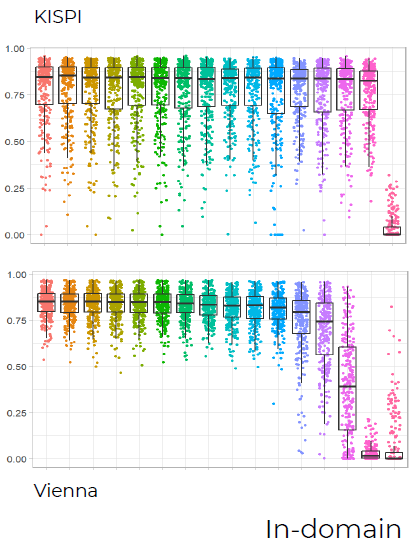
\includegraphics[width=0.4\textwidth]{figures/feta24_in-domain.png}
    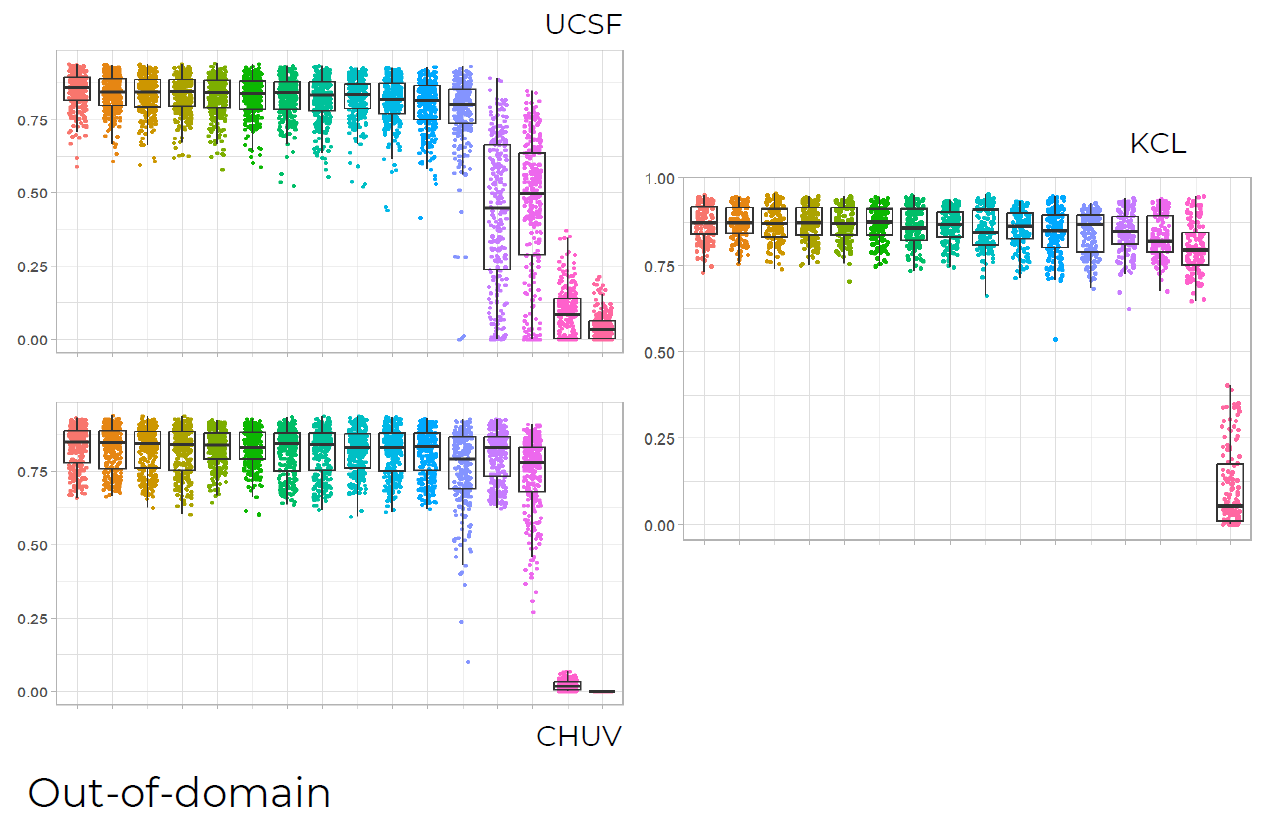
\includegraphics[width=0.8\textwidth]{figures/feta24_out-of-domain.png}
    \caption{Teams' Dice similarity scores in FeTA 2024. From \cite{FeTA2024}.}
    \label{fig:FeTA2024_results}
\end{figure}
